% vim:spelllang=ru,en
\documentclass[a4paper,12pt,notitlepage,headsepline,pdftex]{scrartcl}

\usepackage{cmap} % чтобы работал поиск по PDF
\usepackage[T2A]{fontenc}
\usepackage[utf8]{inputenc}
\usepackage[english,russian]{babel}
\usepackage{concrete}
\usepackage{cite}
\usepackage{url}

\usepackage{textcase}
\usepackage[pdftex]{graphicx}

\usepackage{lscape}

\pdfcompresslevel=9 % сжимать PDF
\usepackage{pdflscape} % для возможности альбомного размещения некоторых страниц
\usepackage[pdftex]{hyperref}
% настройка ссылок в оглавлении для pdf формата
\hypersetup{unicode=true,
            pdftitle={Расчётно-графическая работа по ПО ЭВМ},
            pdfauthor={Погода Михаил},
            pdfcreator={pdflatex},
            pdfsubject={},
            pdfborder    = {0 0 0},
            bookmarksopen,
            bookmarksnumbered,
            bookmarksopenlevel = 2,
            pdfkeywords={},
            colorlinks=true, % установка цвета ссылок в оглавлении
            citecolor=black,
            filecolor=black,
            linkcolor=black,
            urlcolor=blue}

\usepackage{amsmath}
\usepackage{amssymb}
\usepackage{moreverb}
\usepackage{indentfirst}
\usepackage{misccorr}

\usepackage{xtab}
\usepackage{nccfoots}

\usepackage{listings}
\lstloadlanguages{C++}
\lstset{language=C++,basicstyle=\scriptsize,frame=tb,commentstyle=\itshape,stringstyle=\bfseries,extendedchars=false}

\begin{document}
\begin{titlepage}
  \begin{center}
    \large
    \MakeUppercase{Министерство образования и науки,}

    \MakeUppercase{молодёжи и спорта Украины}

    \mbox{\MakeUppercase{Национальный технический университет Украины}}

    \MakeUppercase{,,Киевский политехнический институт''}

    \addvspace{6pt}

    \normalsize
    Кафедра прикладной математики

    \vfill

    \textbf{Расчётно"=графическая работа}

    по дисциплине ,,Программное обеспечение ЭВМ''
  \end{center}

  \vfill

  \noindent
  Выполнил\\
  студент группы КМ-92\\
  Погода~М.\,В.\\
  \vfill

  \vfill

  \begin{center}
    КИЕВ

    2012
  \end{center}
\end{titlepage}
\tableofcontents
\newpage
\section{Введение}
  При сооружении ограждений зачастую решающим фактором является количество
  израсходованных материалов.
  Поэтому желательно использовать такое ограждение, которые бы охватывало всю
  необходимую территорию, и притом длина его была бы оптимальной.

  Самым простым подходом является сооружение ограждение в форме такого
  прямоугольника, который бы касался бы самой нижней, самой верхней, самой
  левой и самой правой точек.
  Тогда, независимо от формы территории, все её точки окажутся внутри этого
  ограждения.

  Однако, этот метод не даёт оптимальную форму ограждения.
  \newpage
\section{Теоретические сведения}
  Как показали исследования, минимальную длину ограждения имеет ограждение в
  форме выпуклой оболочки, построенной для точек территории, которую нужно
  оградить.\cite{book1}

  \emph{Выпуклой оболочкой} множества $\mathbb{X}$ называется наименьшее
  выпуклое множество, содержащее $\mathbb{X}$.
  ,,Наименьшее множество'' здесь означает наименьший элемент по отношению к
  вложению множеств, то есть такое выпуклое множество, содержащее данную
  фигуру, что оно содержится в любом другом выпуклом множестве, содержащем
  данную фигуру.\cite{book2}

  Множество в аффинном пространстве называется \emph{выпуклым}, если оно
  содержит вместе с любыми двумя точками соединяющий их отрезок.

  Существуют несколько методов (алгоритмов), позволяющих построить выпуклую
  оболочку для множества вершин.
  Вот некоторые из них:
  \begin{itemize}
    \item \emph{Алгоритм Грэхема}.
      В этом алгоритме задача о выпуклой оболочке решается с помощью стека,
      сформированного из точек"=кандидатов.
      Все точки входного множества заносятся в стек, а потом точки, не
      являющиеся вершинами выпуклой оболочки, со временем удаляются из него.
      По завершении работы алгоритма в стеке остаются только вершины оболочки
      в порядке их обхода против часовой стрелки.\cite{book3}
    \item \emph{Алгоритм Джарвиса}.
      Метод можно представить как обтягивание верёвкой множества вбитых в
      доску гвоздей.
      Алгоритм работает за время \verb'O(nh)', где \verb'n' --- общее число
      точек на плоскости, \verb'h' --- число точек в выпуклой
      оболочке.\cite{book4}
    \item \emph{Алгоритм Чана}.
      Является комбинацией двух более медленных алгоритмов (сканирование по
      Грэхему  и заворачивание по Джарвису).
      Недостатком сканирования по Грэхему является необходимость сортировки
      всех точек по полярному углу, что занимает достаточно много времени.
      Заворачивание по Джарвису требует перебора всех точек для каждой из
      точек выпуклой оболочки, что в худшем случае занимает квадратичное
      время.\cite{book5}
    \item \emph{Алгоритм быстрой оболочки}.
      Использует идею быстрой сортировки Хоара.
    \item \emph{Алгоритм Киркпатрика}
  \end{itemize}
  \subsection{Описание выбранного метода}
    \emph{Алгоритм Грэхема} --- алгоритм построения выпуклой оболочки в
    двумерном пространстве.
    В этом алгоритме задача о выпуклой оболочке решается с помощью стека,
    сформированного из точек"=кандидатов.
    Все точки входного множества заносятся в стек, а потом точки, не
    являющиеся вершинами выпуклой оболочки, со временем удаляются из него.
    По завершении работы алгоритма в стеке остаются только вершины оболочки в
    порядке их обхода против часовой стрелки.

    \subsubsection{Решение контрольных примеров}
      \paragraph{Пример \No 1}
        \begin{equation*}
          A = \left\{ (0, 0), (1, 0), (2, 0),
                      (0, 1), (1, 1), (2, 1),
                      (0, 2), (1, 2), (2, 2) \right\}
        \end{equation*}

        Отсортируем точки по возрастанию их полярного угла:
        \begin{equation*}
          A_1 = \left\{ (0, 0), (1, 0), (2, 0),
                        (2, 1), (1, 1), (2, 2),
                        (1, 2), (0, 1), (0, 2)\right\}
        \end{equation*}

        Точки $\left\{ (0, 0), (1, 0), (2, 0) \right\}$ лежат на одной прямой,
        поэтому точку $(1, 0)$ можно выбросить из множества точек.
        Точки $\left\{ (0, 0), (2, 0), (2, 1) \right\}$ образуют левый
        поворот, поэтому сохраняем точку $(0, 0)$, рассматриваем точки далее.

        Точки $\left\{ (2, 0), (2, 1), (1, 1)\right\}$ образуют левый поворот,
        поэтому сохраняем точку $(2, 0)$ и рассматриваем точки далее.

        Точки $\left\{ (2, 1), (1, 1), (2, 2) \right\}$ образуют правый
        поворот, поэтому исключаем точку $(1, 1)$ и рассматриваем точки,
        начиная с предыдущей сохранённой.

        Точки $\left\{ (2, 0), (2, 1), (2, 2) \right\}$ лежат на одной прямой,
        поэтому точку $(2, 1)$ можно исключить.

        Точки $\left\{ (2, 0), (2, 2), (1, 2) \right\}$ образуют левый
        поворот, поэтому сохраняем точку $(2, 0)$ и рассматриваем точки далее.

        Точки $\left\{ (2, 2), (1, 2), (0, 1) \right\}$ образуют правый
        поворот, поэтому исключаем точку $(1, 2)$ и рассматриваем точки,
        начиная с предыдущей сохранённой.

        Точки $\left\{ (2, 0), (2, 2), (0, 1) \right\}$ образуют левый
        поворот, поэтому сохраняем точку $(2, 0)$ и рассматриваем точки далее.

        Точки $\left\{ (2, 2), (0, 1), (0, 2) \right\}$ образуют правый
        поворот, поэтому исключаем точку $(0, 1)$ и рассматриваем точки
        начиная с предыдущей сохранённой.

        Точки $\left\{ (2, 0), (2, 2), (0, 2) \right\}$ образуют левый
        поворот, поэтому сохраняем точку $(2, 0)$ и рассматриваем точки далее.

        Т.\,к. больше не осталось не рассмотренных точек, получаем ответ:

        \begin{equation*}
          \mathop{Conv} A = \left\{ (0, 0), (2, 0), (2, 2), (0, 2) \right\}
        \end{equation*}


      \paragraph{Пример \No 2}
        \begin{equation*}
          A = \left\{ (0, 0), (1, 0), (2, 0),
                      (0, 1), (1, 1),
                      (0, 2) \right\}
        \end{equation*}

        Отсортируем точки по возрастанию их полярного угла:
        \begin{equation*}
          \left\{ (0, 0), (1, 0), (2, 0),
                  (1, 1), (0, 1), (0, 2) \right\}
        \end{equation*}

        Точки $\left\{ (0, 0), (1, 0), (2, 0) \right\}$ лежат на одной прямой,
        поэтому точку $(1, 0)$ можно выбросить из множества точек.
        Точки $\left\{ (0, 0), (2, 0), (1, 1) \right\}$ образуют левый
        поворот, поэтому сохраняем точку $(0, 0)$, рассматриваем точки далее.

        Точки $\left\{ (2, 0), (1, 1), (0, 1)\right\}$ образуют левый поворот,
        поэтому сохраняем точку $(2, 0)$ и рассматриваем точки далее.

        Точки $\left\{ (1, 1), (0, 1), (0, 2) \right\}$ образуют правый
        поворот, поэтому исключаем точку $(0, 1)$ и рассматриваем точки,
        начиная с предыдущей сохранённой.

        Точки $\left\{ (2, 0), (1, 1), (0, 2) \right\}$ лежат на одной прямой,
        поэтому точку $(1, 1)$ можно исключить.

        Т.\,к. больше не осталось не рассмотренных точек, получаем ответ:

        \begin{equation*}
          \mathop{Conv} A = \left\{ (0, 0), (2, 0), (0, 2) \right\}
        \end{equation*}

  \newpage
\section{Программная реализация}
  \subsection{Схема взаимодействия подпрограмм}
    \begin{figure}[h]
      \caption{Схема взаимодействия подпрограмм}
      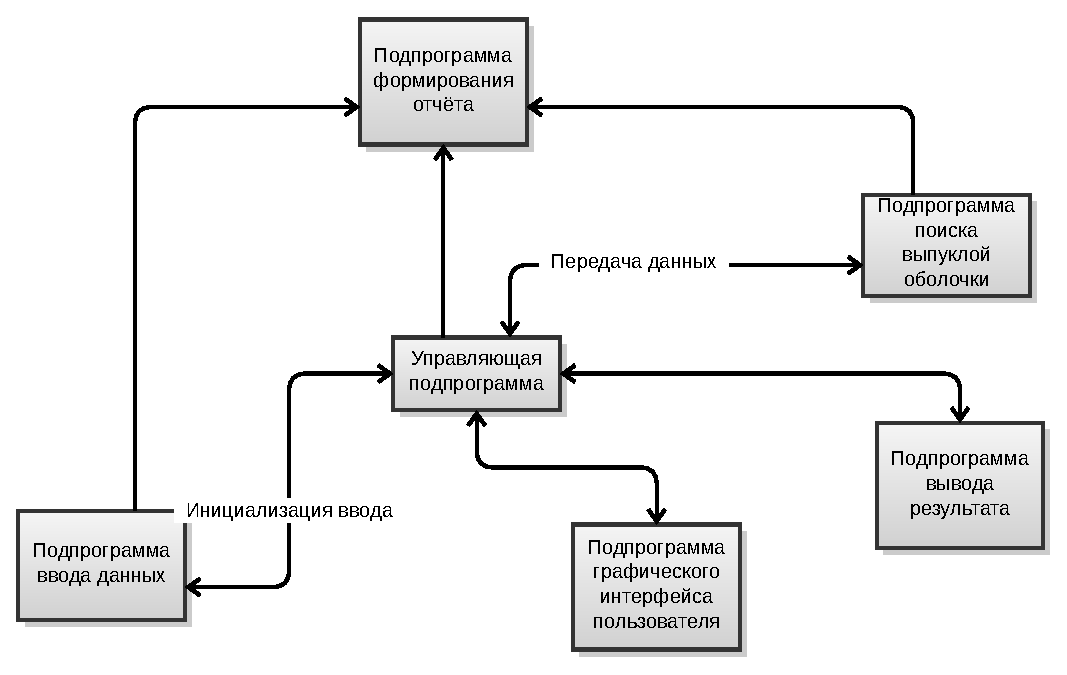
\includegraphics{scheme.eps}
    \end{figure}

    \begin{enumerate}
      \item Управляющая подпрограмма инициирует графический интерфейс и ожидает
        действий пользователя.
      \item Управляющая подпрограмма получает запрос на инициацию действий от
        графического интерфейса.
      \item Управляющая подпрограмма инициирует ввод данных.
      \item Управляющая подпрограмма передаёт исходные данные подпрограмме поиска
        выпуклой оболочки и ожидает результатов вычисления.
      \item Управляющая подпрограмма инициирует вывод данных и графическое
        отображение результата.
      \item Подпрограмма ведение отчёта ожидает сообщений от других подпрограмм.
    \end{enumerate}
  \subsection{Формат исходных данных и результатов работы}
    Поиск выпуклой оболочки на плоскости заключается в выборе из множества всех
    точек таких точек, которые создают выпуклую оболочку этого множества.

    Таким образом,
    \begin{equation}
      \mathop{conv} A : \mathbb{R}^2 \rightarrow \mathbb{R}^2
      \label{eq:1}
    \end{equation}

    Для представления точки на плоскости можно использовать абстрактный тип
    данных, хранящий её координаты.

    Таким образом, программа принимает на вход программа получает множество
    (массив, список, коллекцию) пар вещественных чисел, и возвращает тоже
    множество таких пар.

    Между подпрограммами существуют такие связи:
    \begin{itemize}
      \item Управляющая подпрограмма обрабатывает сигналы от других модулей и
        передаёт им соответствующие сигналы управления;
      \item Подпрограмма ввода принимает сигнал управления и данные, вводимые
        пользователем (список точек либо имя файла, содержащего точки),
        обрабатывает эти данные (распознает вводимые пользователем точки/считывает
        данные из файла) и передаёт управляющей программе множество точек;
      \item Подпрограмма вывода принимает сигнал управления и данные, преобразует
        их в необходимый вид (бинарный/текстовый) и выводит их на устройство
        ввода;
      \item Подпрограмма графического интерфейса пользователя принимает
        управляющие сигналы и различные действия пользователя;
      \item Подпрограмма ведения отчёта принимает сообщения о ходе работы
        программы от других модулей программы, формирует из них отчёт.
    \end{itemize}
  \subsection{Алгоритм работы прикладного программного обеспечения}
    \begin{figure}[h]
      \begin{center}
        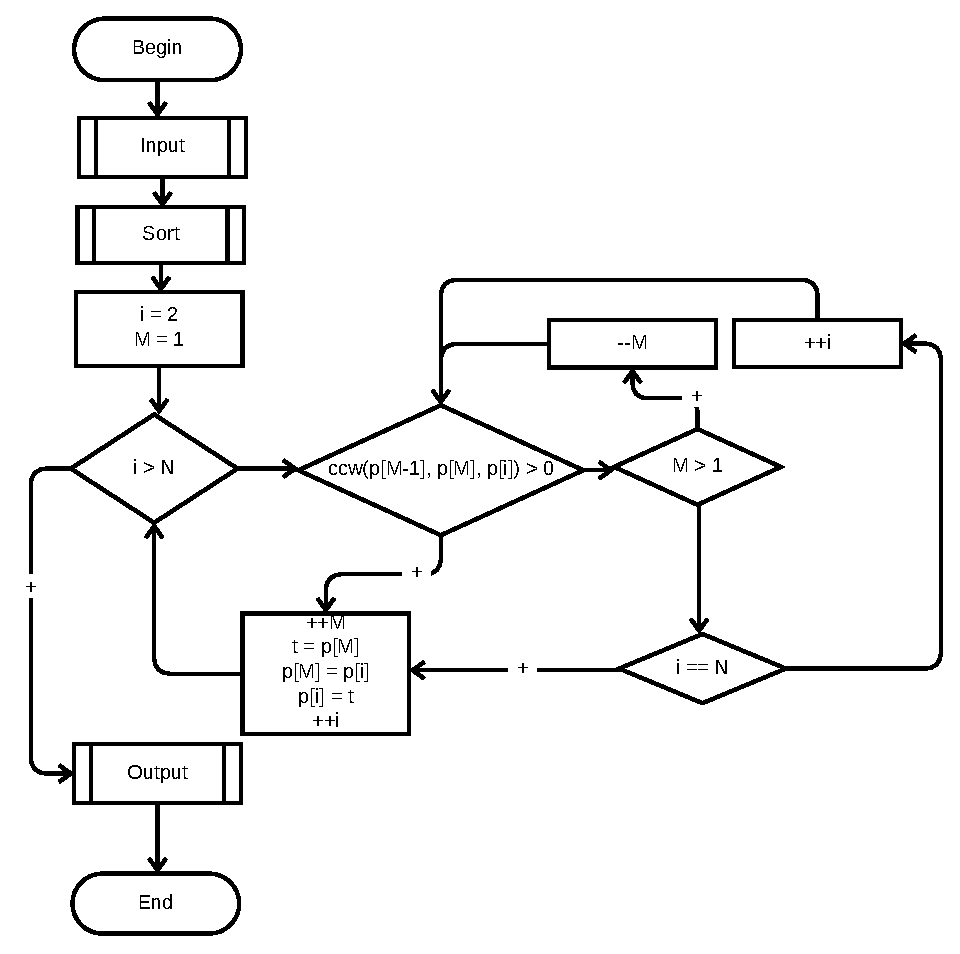
\includegraphics{algo.eps}
      \end{center}
      \caption{Блок"=схема работы алгоритма}
      \label{fig:algo}
    \end{figure}

    \begin{figure}[h]
      \begin{center}
        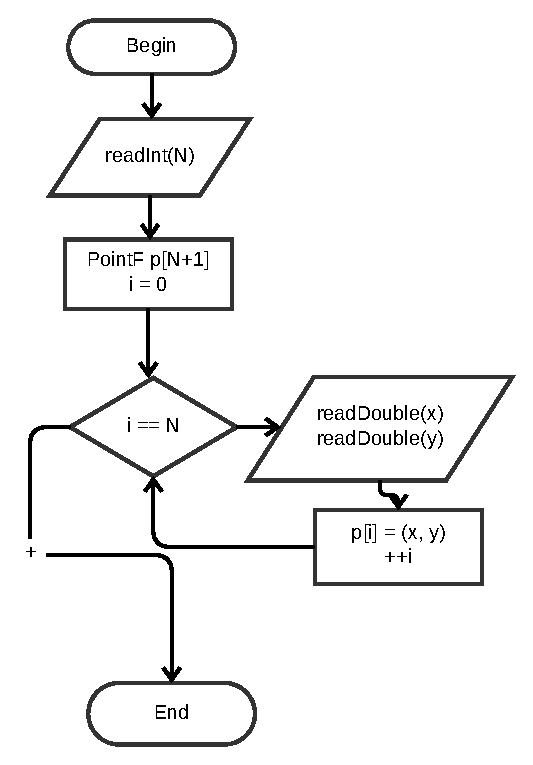
\includegraphics{input.eps}
      \end{center}
      \caption{Блок"=схема ввода данных}
      \label{fig:input}
    \end{figure}

    \begin{figure}[h]
      \begin{center}
        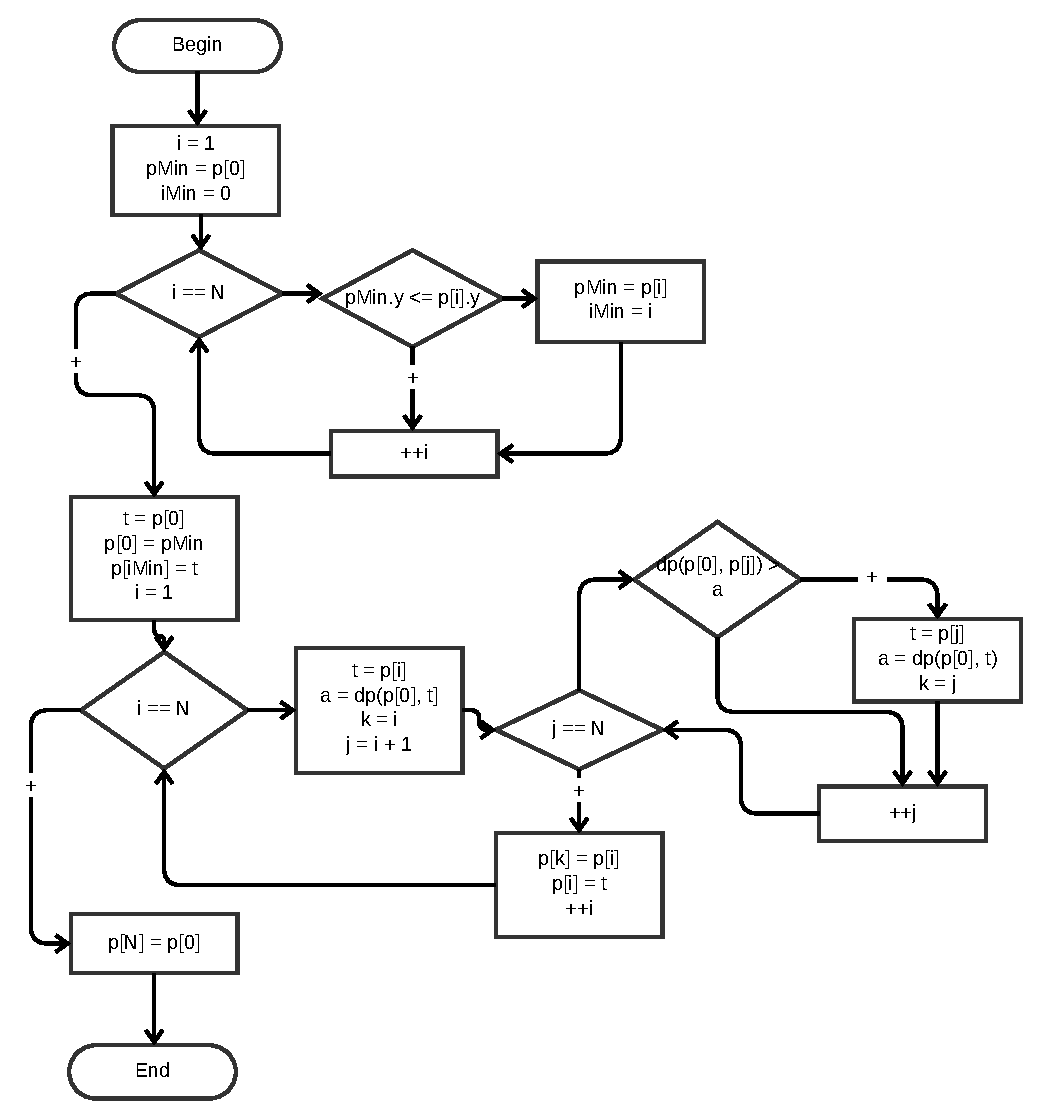
\includegraphics{sort.eps}
      \end{center}
      \caption{Блок"=схема подготовки массива к работе}
      \label{fig:sort}
    \end{figure}

    \begin{figure}[h]
      \begin{center}
        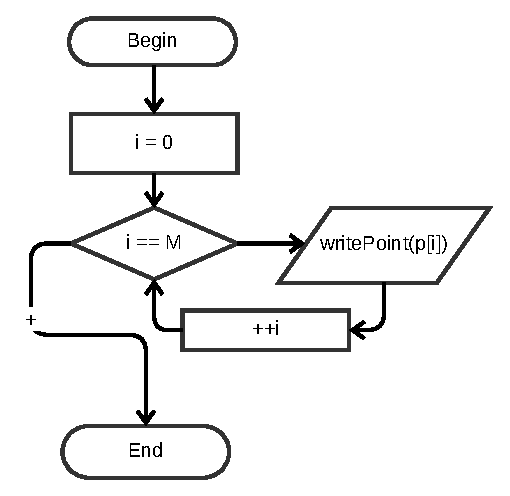
\includegraphics{output.eps}
      \end{center}
      \caption{Блок"=схема вывода результата}
      \label{fig:output}
    \end{figure}
    \clearpage
  \subsection{Реализация алгоритма}
    Для представления точки на плоскости используется АТД\footnote{Абстрактный тип
    данных} \texttt{PointF}, интерфейс которого описан в файле
    \textit{pointf.hxx}, а реализация --- в файле \textit{pointf.cxx}.

    Сама же реализация метода поиска выпуклой оболочки находится в классе
    \texttt{Convex\_Hull} (файлы \textit{convex\_hull.hxx} и
    \textit{convex\_hull.cxx}, см. стр.~\pageref{sec:apcode})
    \newpage

\addcontentsline{toc}{section}{Приложения}
\section*{Приложения}
  \subsection*{Эскиз экранной формы}
  \addcontentsline{toc}{subsection}{Эскиз экранной формы}
    \begin{figure}[h]
      \begin{center}
        %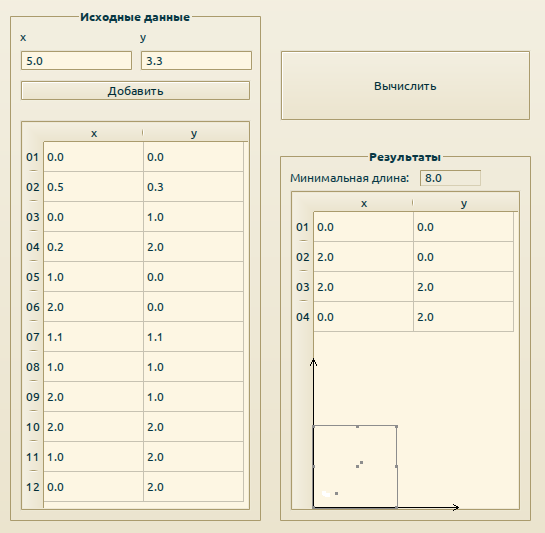
\includegraphics[width=\textwidth]{scr.png}
        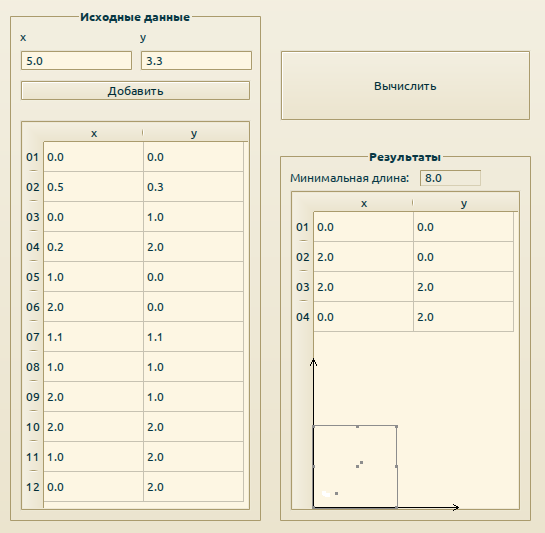
\includegraphics[scale=0.6]{scr.png}
      \end{center}
      \caption{Эскиз экранной формы приложения}
      \label{fig:scr}
    \end{figure}
    \clearpage
  \subsection*{Исходные тексты}
  \addcontentsline{toc}{subsection}{Исходные тексты}
  \label{sec:apcode}
    \subsubsection*{pointf.hxx}
      \lstinputlisting{pointf.hxx}
    \subsubsection*{pointf.cxx}
      \lstinputlisting{pointf.cxx}
    \subsubsection*{convex\_hull.hxx}
      \lstinputlisting{convex_hull.hxx}
    \subsubsection*{convex\_hull.cxx}
      \lstinputlisting{convex_hull.cxx}

      \clearpage
  \addcontentsline{toc}{subsection}{Список литературы}
    \bibliographystyle{ugost2008ls}
    \bibliography{src}
\end{document}
